\section{RFC-0013: Return path
incentivization}\label{rfc-0013-return-path-incentivization}

\begin{itemize}
\tightlist
\item
  \textbf{RFC Number:} 0013
\item
  \textbf{Title:} Return path incentivization
\item
  \textbf{Status:} Raw \textbar{} Discussion \textbar{} Prototype
  \textbar{} Implementation \textbar{} Finalized \textbar{} Rejected
  \textbar{} Superseded
\item
  \textbf{Author(s):} \textless Name (GitHub Handle)\textgreater{}
\item
  \textbf{Created:} \textless YYYY-MM-DD\textgreater{}
\item
  \textbf{Updated:} \textless YYYY-MM-DD\textgreater{}
\item
  \textbf{Version:} v0.x.x (Raw), v1.x.x (Finalized)
\item
  \textbf{Supersedes:} RFC-YYYY (if applicable)
\item
  \textbf{Related Links:} {[}Related RFCs or Documentation Links{]}
\end{itemize}

\subsection{1. Abstract}\label{1-abstract}

Provide a brief and clear summary of the RFC, outlining its purpose,
context, and scope.

\subsection{2. Motivation}\label{2-motivation}

Explain the problem this RFC aims to solve. Discuss existing
limitations, technical gaps, and why the proposed solution is necessary.

\subsection{3. Terminology}\label{3-terminology}

Define key terms, abbreviations, and domain-specific language used
throughout the RFC.

\subsection{4. Specification}\label{4-specification}

Comprehensive description of the proposed solution, including:

\begin{itemize}
\tightlist
\item
  Protocol overview
\item
  Technical details (data formats, APIs, endpoints)
\item
  Supported use cases
\item
  Diagrams (stored in \texttt{assets/} and referenced as
  \texttt{!{[}Diagram{]}(assets/diagram-name.png)})
\end{itemize}

\pandocbounded{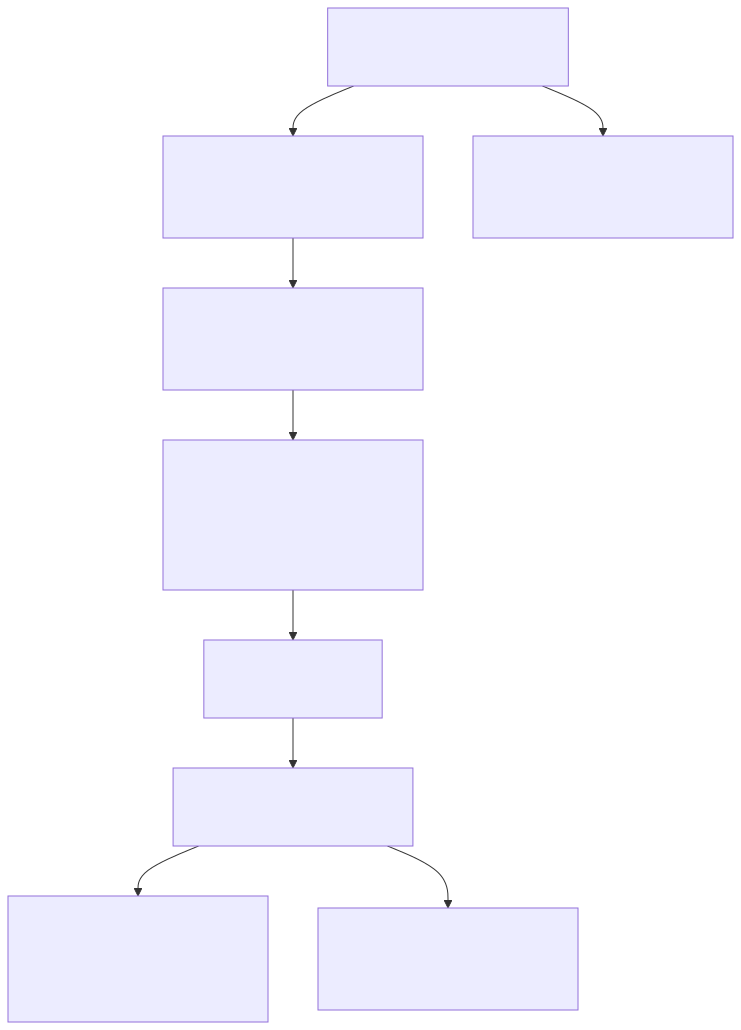
\includegraphics[keepaspectratio,width=\maxwidth,alt={Mermaid Diagram 1}]{generated/0013-return-path-incentivization/mermaid_1.png}}

\subsection{5. Design Considerations}\label{5-design-considerations}

Discuss critical design decisions, trade-offs, and justification for
chosen approaches over alternatives.

\subsection{6. Compatibility}\label{6-compatibility}

Address backward compatibility, migration paths, and impact on existing
systems.

\subsection{7. Security Considerations}\label{7-security-considerations}

Identify potential security risks, threat models, and mitigation
strategies.

\subsection{8. Drawbacks}\label{8-drawbacks}

Discuss potential downsides, risks, or limitations associated with the
proposed solution.

\subsection{9. Alternatives}\label{9-alternatives}

Outline alternative approaches that were considered and reasons for
their rejection.

\subsection{10. Unresolved Questions}\label{10-unresolved-questions}

Highlight questions or issues that remain open for discussion.

\subsection{11. Future Work}\label{11-future-work}

Suggest potential areas for future exploration, enhancements, or
iterations.

\subsection{12. References}\label{12-references}

Include all relevant references, such as:

\begin{itemize}
\tightlist
\item
  Other RFCs
\item
  Research papers
\item
  External documentation
\end{itemize}
